\section{Experimental Results}
\label{sec:clgen-eval-results}

The effectiveness of synthetic benchmarks is evaluated on two heterogeneous systems. First, the performance of a state-of-the-art predictive model~\cite{Grewe2013} is compared with and without the addition of synthetic benchmarks, then synthetic benchmarks are shown to expose weaknesses in the feature design and how these can be addressed to develop a better model. Finally, the ability of CLgen to explore the program feature space is compared against a state-of-the-art program generator.

\subsection{Performance Evaluation}

\begin{figure}
  \centering %
  \subfloat[][AMD Tahiti 7970]{%
    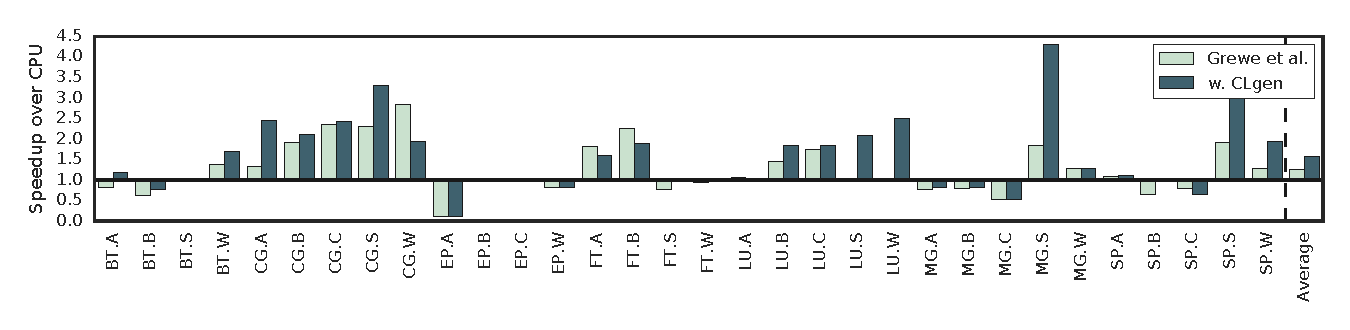
\includegraphics[width=.32\textwidth,angle=0]{img/ex1-A}%
    \label{fig:npb-amd}}%
  \subfloat[][NVIDIA GTX 970]{%
    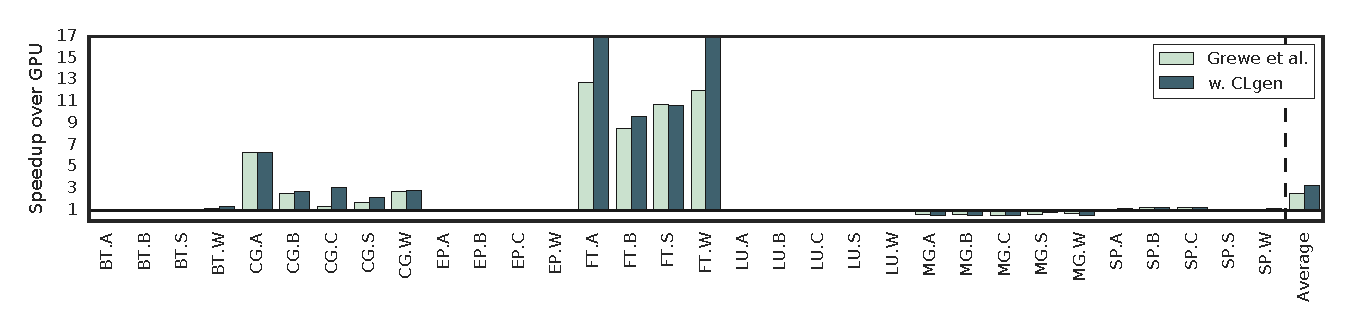
\includegraphics[width=.32\textwidth,angle=0]{img/ex1-B}%
    \label{fig:npb-nvidia}}%
  \caption[Speedup of predictions with and without synthetic benchmarks]{%
    Speedup of programs using \citeauthor{Grewe2013} predictive model with and without synthetic benchmarks. The predictive model outperforms the best static device mapping by a factor of $1.26\times$ on AMD and $2.50\times$ on NVIDIA. The addition of synthetic benchmarks improves the performance to $1.57\times$ on AMD and $3.26\times$ on NVIDIA.%
  }%
  \label{fig:npb} %
\end{figure}

Figure~\ref{fig:npb} shows speedups of the \citeauthor{Grewe2013} predictive model over the NAS Parallel Benchmark suite with and without the addition of synthesised benchmarks for training. Speedups are calculated relative to the best single-device mapping for each experimental platform, which is CPU-only for AMD and GPU-only for NVIDIA. The fine-grained coverage of the feature space which synthetic benchmarks provide improves performance dramatically for the NAS benchmarks. Across both systems, an average speedup of $2.42\times$ is achieved with the addition of synthetic benchmarks, with prediction improvements over the baseline for 62.5\% of benchmarks on AMD and 53.1\% on NVIDIA.

The strongest performance improvements are on NVIDIA with the \texttt{FT} benchmark which suffers greatly under a single-device mapping. However, the performance on AMD for the same benchmark slightly degrades after adding the synthetic benchmarks. This issue is addressed in the next section.

\subsection{Extending the Predictive Model}
\label{subsec:eval-extended}

Feature designers are bound to select as features only properties which are significant for the handful of benchmarks they test on, which limits a model's ability to generalise over a wider range of programs. This is found to be the case with the \citeauthor{Grewe2013} model. The addition of automatically generated programs exposed two distinct cases where the model failed to generalise as a result of overspecialising to the NPB suite.

The first case is that the feature \texttt{F3} of Table~\ref{tab:clgen-cgo13-features} is sparse on many programs. This is a result of the NPB implementation's heavy exploitation of local memory buffers and the method by which they combined features (speculatively, this may have been a necessary dimensionality reduction in the presence of sparse training programs). A simple countermeasure is taken to address this by extending the model to use the raw feature values in addition to the combined features.

The second case is that some CLgen-generated programs had identical feature values as in the benchmark set, but had different \emph{behaviour} (i.e. optimal mappings). Listing~\ref{lst:zero-b} shows one example of a CLgen benchmark which is indistinguishable in the feature space to one the of existing benchmarks --- AMD's Fast Walsh-Hadamard transform, Listing~\ref{lst:amd-fast-walsh-transform} --- but with different behaviour. We found this to be caused by the lack of discriminatory features for branching, since the NPB programs are implemented in a manner which aggressively minimised branching. To counter this the predictive model was extended with an additional feature containing a static count of branching operations in a kernel.

\begin{listing}
  \inputminted{opencl_lexer.py:OpenCLLexer -x}{lst/amd-fast-walsh-transform.cl}
  \caption[AMD's Fast Walsh Transform kernel]{AMD's Fast Walsh Transform benchmark kernel. In the \citeauthor{Grewe2013} feature space this is indistinguishable from the CLgen program of Listing~\ref{lst:zero-b}, but has very different runtime behaviour and optimal device mapping. The addition of a branching feature fixes this.}
  \label{lst:amd-fast-walsh-transform}
\end{listing}

\begin{listing}
  \inputminted{opencl_lexer.py:OpenCLLexer -x}{lst/amd-fast-walsh-transform-equivalent.cl}
  \caption[Synthesised program with same features as an AMD benchmark]{In the \citeauthor{Grewe2013} feature space, this CLgen program is indistinguishable from the AMD Fast Walsh–Hadamard transform benchmark kernel of Listing~\ref{lst:amd-fast-walsh-transform}, but has very different runtime behaviour and optimal device mapping. The addition of a branching feature fixes this.}
  \label{lst:zero-b}
\end{listing}

Figure~\ref{fig:ex2} shows speedups of the extended model across all seven of the benchmark suites used in Section~\ref{sec:the-case-for-benchmark-generators}. Model performance, even on this tenfold increase of benchmarks, is good. There are three benchmarks on which the model performs poorly: \texttt{MatrixMul}, \texttt{cutcp}, and \texttt{pathfinder}. Each of those programs makes heavy use of loops, which changes the dynamic behaviour of the programs in ways that the static code features of the model are unlikely to capture. This could be addressed by extracting dynamic instruction counts using profiling, but this is beyond the scope of this work. It is not the aim of this work to perfect the predictive model but to show the performance improvements associated with training on synthetic programs. To this extent, the proposed approach succeeds, achieving average speedups of $3.56\times$ on AMD and $5.04\times$ on NVIDIA across a very large test set.

\begin{figure}
  \centering%
  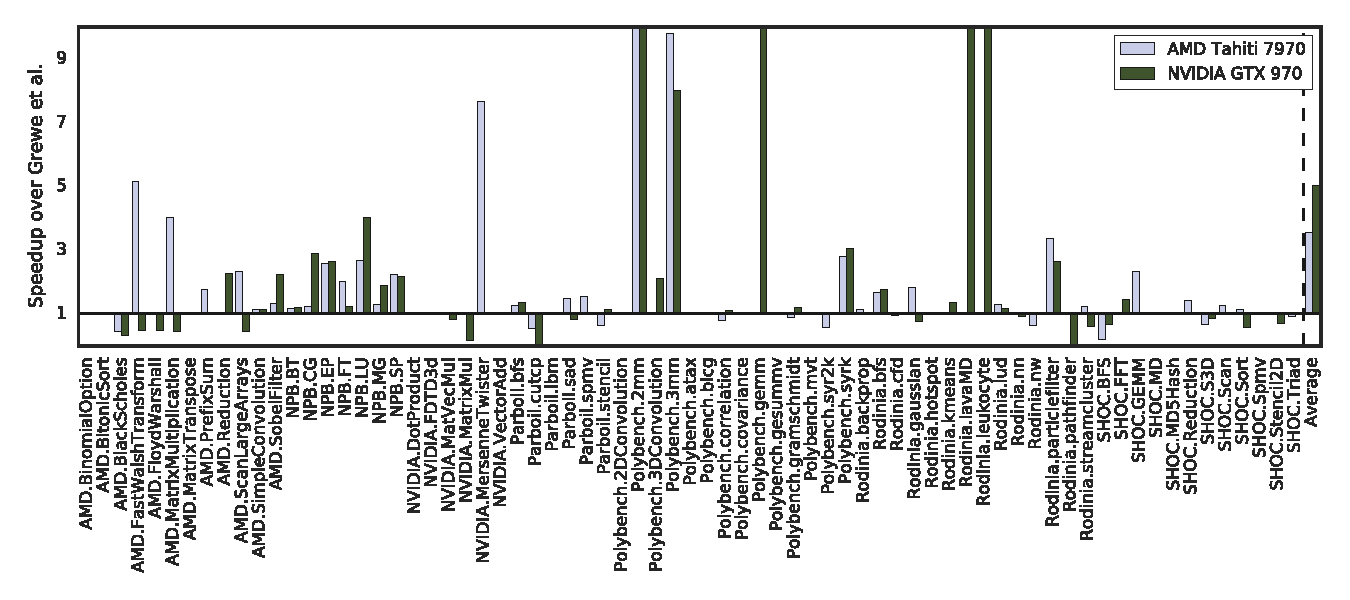
\includegraphics[width=1.45\textwidth,angle=270]{img/ex2}%
  \caption[Speedups of predictions using extended model over state-of-the-art]{%
    Speedups of predictions using an extended model over \citeauthor{Grewe2013} on both experimental platforms. Synthetic benchmarks and the additional program features outperform the original predictive model by a factor $3.56\times$ on AMD and $5.04\times$ on NVIDIA.%
  }%
  \label{fig:ex2}%
\end{figure}


\subsection{Comparison of Source Features}

As demonstrated in Section~\ref{sec:the-case-for-benchmark-generators}, the predictive quality of a model for a given point in the feature space is improved with the addition of observations from neighbouring points. By producing thousands of artificial programs modelled on the structure of real OpenCL programs, CLgen is able to consistently and automatically generate programs which are close in the feature space to the unseen benchmarks that are in the test set.

To quantify this effect, the static code features of Table~\ref{tab:clgen-cgo13-features-raw}, plus the branching feature discussed in the previous subsection, are used to measure the number of CLgen kernels generated with the same feature values as those of the benchmarks examined in the previous sections. Only static code features are examined to allow comparison with the GitHub kernels for which there is no automated method to execute and extract runtime features, and programs generated by CLSmith.

Figure~\ref{fig:clgen-nearest-neighbour} plots the number of exact feature vector matches as a function of the number of kernels. Out of 10,000 unique CLgen kernels, more than a third have static feature values matching those of the benchmarks, providing on average 14 CLgen kernels for each benchmark. This supports the underlying intuition: CLgen kernels, by emulating the way real humans write OpenCL programs, are concentrated in the same area of the feature space as real programs. Moreover, since the number of CLgen kernels that can be generated is unbounded, the exploration of the feature space can be continually refined. This is not the case for GitHub, where the number of kernels is finite. CLSmith rarely produces code similar to real-world OpenCL programs, with only 0.53\% of the generated kernels have matching feature values with benchmark kernels. The unique contribution of CLgen is its ability to generate many thousands of programs \textit{that are appropriate for predictive modelling}.

\begin{figure}
  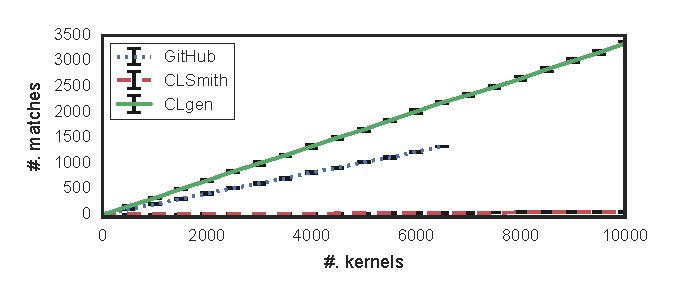
\includegraphics[width=\columnwidth]{img/closeness} %
  \caption[Number of kernels matching benchmark features]{%
    The number of kernels from GitHub, CLSmith, and CLgen with static code features matching the benchmarks. CLgen generates kernels that are closer in the feature space than CLSmith, and continues to do so long after the extent of the GitHub data set is exhausted. Error bars show the standard deviation from 10 random samplings.%
  }%
  \label{fig:clgen-nearest-neighbour}
\end{figure}
